%%%%%%%%%%%%%%%%%%%%%%%%%%%%%%%%%%%%%%%%%%%%%%%%%%%%%%%%%%%%%%%%%%%%%%%%%%%%%%%
%%	PARA INSERTAR FIGURAS USAR LA FUNCION PREDEFINIDA \imagen
%%
%%      \imagen{escala}{path imagen}{caption}{referencia}
%%
%% donde:
%% 	* escala: es un valor numérico. Preferentemente usar valores entre 0 y 1.
%%		(ejemplo: 0.2)
%% 	* path: imagen es el directorio relativo donde se encuentra la imagengit 
%%		(ejemplo: Figures/Logos/conae-logo.png)
%%	* caption: texto de pie de figura.
%%	* referencia: texto que sirve para citar la figura. 
%%		(ejemplo: fig:conaelogo) luego se podrá hacer referencia \ref{fig:conaelogo}
%%%%%%%%%%%%%%%%%%%%%%%%%%%%%%%%%%%%%%%%%%%%%%%%%%%%%%%%%%%%%%%%%%%%%%%%%%%%%%%

%------------------------------------------------------------------------------
% Formato del documento
\documentclass[11pt, a4paper, twoside]{report}

%------------------------------------------------------------------------------
% TEMPLATE MDIAE (ACÁ SE ENCUETRAN LAS CUSTOMIZACIONES)
% Remitirse al archivo mdiaedoc.sty
\usepackage{mdiaedoc}

%Configuración de los márgenes
\usepackage[top=3cm, bottom=3cm, left=2.5cm, right=1.5cm]{geometry}

\usepackage{natbib}
\usepackage{import}

% Para gráficos
\usepackage{tikz}
\usetikzlibrary{shapes,snakes}
\usetikzlibrary{arrows,positioning} 
\usetikzlibrary{babel}

%------------------------------------------------------------------------------
% Esto no se usa (YA ESTA DEFINIDO EN EL TEMPLATE)
%\usepackage{setspace}

%%%%%%%%%%%%%%%%%%%%%%%%%%%%%%%%%%%%%%%%%%%%%%%%%%%%%%%%%%%%%%%%%%%%%%%%%%%%%%%
% COMIENZO DEL DOCUMENTO
%%%%%%%%%%%%%%%%%%%%%%%%%%%%%%%%%%%%%%%%%%%%%%%%%%%%%%%%%%%%%%%%%%%%%%%%%%%%%%%
\begin{document}

\makeatletter
\author{Arias Emmanuel}
\makeatother

%------------------------------------------------------------------------------
% PORTADA
\portadatesis{Diseño de una arquitectura de aviónica tolerante a fallas basada en componentes COTS para vehículos
satelitales de nueva generación}{Arias Emmanuel}{UNIVERSIDAD NACIONAL DEL CÓRDOBA}{Mayo, 
2017}{2017}{Gustavo Wiman}{INVAP, Bariloche, Provincia de Rio Negro}

%------------------------------------------------------------------------------
% EN CASO DE TENER UN ASESOR CIENTIFICO, DESCOMENTAR LO SIGUIENTE 
% \begin{center}
% \normalsize ASESOR CIENTÍFICO:\\
% \normalsize \textit{\textbf{Nombre del asesor}}\\
% \end{center}

%------------------------------------------------------------------------------
% COMPLETAR CON LICENCIA CREATIVE COMMONS SEGÚN CORRESPONDA
%\begin{center}
%%%%% Ejemplo %%%%%%
%\begin{figure}[H]
%    \centering
%    \includegraphics[width=3cm, keepaspectratio=true]{imagenes/Logos/creativecommons.png}
%\end{figure}
%\vspace*{-0.5cm}
%Esta obra está bajo una \href{http://creativecommons.org/licenses/by-sa/2.5/ar/}{Licencia Creative Commons Atribución-CompartirIgual 2.5 Argentina.}
%\end{center}

\pagenumbering{gobble}

\chapter*{}
\begin{flushright}
  \textit{
    A mi madre, \\
    gracias a tus palabras \\
    mirá a dónde llegué. Y no me detendré. 
  }
\end{flushright}

\chapter*{Abstract}
\label{chap:abstract}
The space missions development involves costs of major magnitude, the most important costs
being the development, and the materials used for the manufacture of satellites. The high
cost of these materials is because they are manufactured exclusively for their application
to space activity, that mean that they are "qualified to fly." There are other components
called COTS (Commercial Off-The-Shelf). These COTS components are considerably more
economical than the "classic" ones, thus helping to significantly reduce costs. This is
important to the Argentinian space industry. To achieve a correct application of these
components, it is necessary develop  techniques, strategies and architectures that ensure
that the probability of catastrophic failure and degradation are compatible with the mission.
In this work, we firstly studied and proposed models of different topologies that will
be used to develop a fault tolerant architecture based on COTS components. Then, a communication
protocol called CANae is developed. CANae is  based on the CAN (Controller Area Network)
protocol, and CANae is oriented to work in distributed networks. Finally, in this thesis
be proposed an architecture based on both COTS components and distributed networks, that
uses the protocol CANae for the communication with its components. In this way, an
architectural proposal is developed to ensures that the system is reliable, even though
the components that make it up are of low reliability.


\textbf{Keywords: COTS Components, Fault Tolerant Architecture, Avionics, Fault Tolerance, Satellites}

\chapter*{Resumen} % si no queremos que añada la palabra "Capitulo"
%\addcontentsline{toc}{chapter}{Resumen} % si queremos que aparezca en el índice

Esta tesis se trata de
\chapter*{Agradecimientos}
\label{chap:agradecimientos}
%\addcontentsline{toc}{chapter}{Agradecimientos}
Muchas gracias
 %% OPCIONAL

\tabladecontenidos

\chapter*{Lista de acrónimos}
\label{chap:acronimos}
\begin{acronym}[TESIS]
\acro{SW}{Software}
\acro{FT}{Tolerancia a Fallas}
\acro{FA}{Evitación de Fallas}
\acro{FR}{Eliminación de Fallas}
\acro{FF}{Predicción de Fallas}
\acro{MTBF}{Tiempo Medio Entre Fallas}
\acro{MTTF}{Tiempo Medio de Fallas}
\acro{MTTR}{Tiempo Medio de Reperación}
\acro{CMF}{Modo Común de fallas}
\acro{FDIR}{Detección, Aislación y Recuperación de Fallas}
\acro{CONAE}{Comisión Nacional de Actividades Espaciales}
\acro{UNLAM}{Universidad Nacional de La Matanza}
\acro{INVAP}{Investigación Aplicada}
\acro{NASA}{National Aeronautics and Space Administration}
\acro{COTS}{Commercial Off-The-Shelf}
\end{acronym}

%------------------------------------------------------------------------------
% Numeración arábiga a partir de este punto
\section{Introducción}
Los proyectos aeroespaciales emplean una arquitectura de aviónica que se denomina \textbf{federada}, en la cual cada computadora del sistema se diseña para que desarrolle una sola función específica \citep{Loveless15}. Esta estrategia de diseño tiene varias ventajas, por tal motivo ha sido utilizada a lo largo de los años. En contraposición, cuenta con varias desventajas, que alientan al surgimiento de nuevas formas de pensamiento y desarrollo de aviónica de sistemas espaciales. Algunas de estas desventajas que ya fueron mencionadas con anterioridad son la masa y una utilización ineficiente de los procesadores. Para ello se está comenzando a desarrollar arquitecturas con el paradigma IMA.

\pagenumbering{arabic}
\setcounter{page}{1}

% Marco Teorico
\chapter{Marco Teórico}\label{chap:marco_teorico}
% section that talk about terminology
% esta seccion habla sobre los términos importantes a utilizar a lo largo de la tesis
\section{Terminología}\label{sec:terminologia}
Existe una importante diferencia entre los significados de las palabras falla, error y
avería\footnote{En inglés: fault, error y failure.}, que es importante destacar. Teniendo en cuenta 
el Diccionario de Cambridge \citep{CambridgeDictionary}\footnote{\texttt{{https://dictionary.cambridge.org/}}}
el significado de fault es, ``1. something that is wrong with something; 2. an imperfection, something wrong;
3. a mistake, especially something for which you are to blame'', 
que se adapta de mejor manera con la palabra española ``falla'', que según la Real Academia Española \citep{RAE}\footnote{\texttt{{http://www.rae.es/}}} es, ``1. defecto o falta; 2. incumplimiento de una
obligación''.  Por otro lado, Failure según \cite{CambridgeDictionary} es, ``1. the fact of someone or something not succeeding; 2. the fact of not doing something that you must do or are expected to do'', que 
nuevamente se adapta mejor con la palabra española ``avería'', la cual significa: ``1. Daño que impide el funcionamiento de un aparato, instalación, vehículo, etc.'' Por esto, en esta obra se utilizan las palabras: falla, error y avería, para las traducciones de fault, error y failure.

Una \textbf{avería} de sistema ocurre cuando el servicio prestado por el sistema ya no coincide con
las especificaciones del mismo \citep{Hanmer07}. Esto quiere decir que existe un problema que tiene
una consecuencia negativa en el sistema completo, logrando que este ya no logre cumplir con sus
especificaciones. Cuando el sistema no se comporta de la manera que es especificada, este ha
fracasado. Esto significa que lo que se espera de un sistema se encuentra descripto, comúnmente en
especificaciones o requerimientos \citep{Pullum01}.

Para la \cite{IEEE610.12} avería es ``la inhabilitación de una sistema o componente a llevar a
cabo las funciones requeridas en los requerimientos específicos de perfomance del mismo''.

\cite{Hanmer07} ejemplifica averías de sistemas cuando: el sistema se bloquea y se detiene cuando no
debería hacerlo, el sistema calcula un resultado incorrecto, el sistema no está disponible, o el
sistema es incapaz de responder a la interacción con el usuario. Cuando el sistema no hace lo que
debe hacer, el sistema ha fracasado. Las averías son detectados por los usuarios mientras usan el
sistema.

Las averías son causados por los errores. Un \textbf{error} es una parte del estado del sistema
que es susceptible de provocar un avería en el sistema. Un error que afecta al servicio, es una
indicación de que una avería se ha producido \citep{Hanmer07}. Un error se puede propagar, es decir
dar a lugar otros errores \citep{Pullum01}.

\cite{IEEE610.12} define error como ``la diferencia entre un valor computado, observado o medido,
con el valor verdadero, especificado o el teóricamente verdadero''.

Según \cite{Rani11} un error es la parte de estado del sistema que puede conducir a una avería, es una
etapa intermedia entre fallas y averías.

Los errores se pueden clasificar en dos tipos: errores de tiempo y valores \citep{Hanmer07}. Los
errores de valores son aquellos que se manifiestan como valores discretos incorrectos o estados del
sistema incorrecto. En cambio, los errores de tiempo pueden incluir aquellos que no cumplen con el total de las tareas.

\cite{Hanmer07} especifica los siguiente casos más comunes de errores:
\begin{itemize}
 \item Timing: existe una falta de sincronización en la comunicación de los procesos.
 \item Bucles infinitos: ejecución de un bucle sin detenerse, esto consume memoria, y la
avería del sistema.
 \item Error de protocolo: errores en el flujo de comunicación ya que no coinciden los
protocolos. Mensajes enviados en formato diferente, en tiempos diferentes, a lugares de sistemas
incorrectos.
 \item Inconsistencia de datos: los errores son diferentes en diferentes lugares.
 \item Sobrecarga de sistema: el sistema es incapaz de hacer frente a la sobrecarga de
actividades a la que es expuesta.
\end{itemize}

La causa adjudicada o la hipótesis de un error es una \textbf{falla}, también llamado ``bugs''. Una
\textbf{falla activa} es aquella que produce un error \citep{Pullum01}. Una falla es un defecto que está
presente en el sistema y que puede causar un error \citep{Hanmer07}. Es la desviación actual de lo
correcto \citep{Hanmer07} \citep{Rani11}. 

Según \cite{IEEE610.12} una falla es ``un defecto en un dispositivo de hardware o componente; como
por ejemplo un corto circuito o un cable cortado''. También realiza una segunda definición diciendo
que falla es ``un paso incorrecto, proceso, o definición de dato en un programa de computadora''
\citep{IEEE610.12}. Esta última afirmación es la que se usa en el ámbito de este trabajo.

Se puede indicar que un software contiene falla, si dado un conjunto de entradas, se obtienen
resultados que son incorrectos. Una falla es una parte del software, y puede ser eliminada mediante 
la corrección de dicha parte. \citep{XIE}

Debe realizar la distinción entre fallas activas y pasivas. Las primeras son aquellas que han sido descubiertas por algún, es decir, mediante testing o durante el funcionamiento del sistema. Si el sistema no es capaz de identificar la falla, aislar y recuperarse de esta, podría llegar a convertirse en una avería. Por otro lado, las fallas pasivas son aquellas que se encuentran dentro del sistema, pero todavía no ha sido detectada, es decir, que no causa ningún efecto observable eternamente (a nivel de sistema). Debe aclararse que una falla se manifieste o no, depende de lo que esté sucediendo en le sistema y su entorno. 

Algunas fallas introducidas en el \ac{SW} se detallan en \cite{Hanmer07}, lo cual señala que
pueden incluir:
\begin{itemize}
 \item Especificaciones incorrecta de requerimientos
 \item Diseño incorrecto
 \item Errores de programación
\end{itemize}


Resumiendo, la principal diferencia entre falla (fault) y avería (failure) es que la primera, es 
la causa de la segunda. Debido a la existencia de una falla, las entradas del módulo (o sistema) software
que contiene dicha falla, provocará como salida valores y/o resultados incorrectos, es decir, 
que no corresponden con los valores teóricos. Por otro lado una avería, es la consecuencia de una falla, 
y se refiere a cuando el sistema deja de responder o comportarse como debería hacerlo, desviándose 
de sus requerimientos. 

Entonces, como lo indica \cite{Pullum01} con la tolerancia a fallas, lo que se busca es prevenir la
avería mediante la ``tolerancia'' de fallas, las cuales son detectables cuando un error aparece.
Las fallas son el motivo de errores y los errores son motivos de avería \citep{FTDesign}.

También se suele utilizar el término anomalía en las operaciones de vehículos espaciales para
referirse a comportamientos anómalos o no esperados del sistema \citep{SpaceSystemFailures}

En \cite{FTDesign} se describe un ejemplo para diferenciar correctamente estos conceptos. Se considera
el \ac{SW} de una planta nuclear, en la cual existe una computadora que es responsable de controlar
la temperatura, la presión y demás variables de interés para la seguridad del sistema. Se da el
caso de que uno de los sensores detecta que la turbina principal se encuentra girando a una
velocidad menor a la correcta. Esta falla hace que el sistema envíe una señal para aumentar su
velocidad (error). Esto produce un exceso de velocidad en la turbina, lo cual tiene como
consecuencia que la seguridad mecánica apague la turbina. En esta situación el sistema no está
generando energía. Esto se considera un avería, porque el sistema no está entregando el servicio
según lo establecido por los requerimientos. Pero es un avería salvable.

Otro concepto es el de \textbf{mantenibilidad}, esta es la capacidad de un sistema, bajo condiciones normales, de ser restaurado a un estado en el cual puede realizar sus funciones requeridas, cuando se realiza el mantenimiento \citep{Rausand04}.

En secciones posteriores se ven los conceptos de confiabilidad, disponibilidad y seguridad (Sección \ref{subsec:confiabilidad}, \ref{subsec:disponibilidad}, \ref{subsec:seguridad}, respectivamente).


% Section that talk about dependability on software
% TODO:La fiabilidad en el software
\section{La fiabilidad en el software}\label{sec:fiabilidad_software}
El objetivo final de la \ac{FT}, es el desarrollo de un sistema fiable \citep{FTDesign}. Teniendo
en cuenta que el \ac{SW} que se encuentra dentro de las naves espaciales, como satélites,
lanzadores, y sobre todo vehículos tripulados son críticos, ya que de ellos dependen el éxito o
fracaso de una misión o la vida de seres humanos,y por lo tanto, se debe llevar a cabo un sistema fiable.
La fiabilidad de un sistema es la capacidad del mismo de entregar a los usuarios un nivel
deseado de servicio \citep{FTDesign}.

La fiabilidad también se la puede considerar como una propiedad global que permite justificar la
confianza de los servicios de un sistema \citep{FTAvionics}. Por lo tanto, como lo indica
\cite{FTAvionics} la fiabilidad es un término amplio y cualitativo que está relacionado con
atributos no funcionales (o ``-ilities''), que buscan generar un sistema ``ideal'', especialmente
cuando su funcionamiento es crítico.

Como se muestra en la Figura \ref{fig:dependability_relations} la consecuencia de la fiabilidad es
la relación entre la evitación de fallos y la reducción de fallos, así como también la \ac{FT}.

\begin{figure}[h]
 \centering
 \includegraphics[scale=0.5]{images/Marco_teorico/dependability_relations}
  \caption{Fiabilidad \protect\citep{FTAvionics}}
\label{fig:dependability_relations}
\end{figure}

Según \cite{Pullum01} la fiabilidad puede ser clasificada en:
\begin{itemize}
 \item Impedimentos: son aquellas cosas que se interponen en el camino de la fiabilidad. Son las
fallas, errores y averías.
 \item Medios: los medios para lograr la fiabilidad, según el autor, se pueden dividir en dos
grupos:
  \begin{enumerate}
    \item Aquellos que son utilizados durante la construcción del \ac{SW} (\ac{FA}\footnote{En
    inglés, Fault Avoidance} y \ac{FT}).
    \item Aquellos que contribuyen con la validación del \ac{SW} una vez desarrollado
    (\ac{FR}\footnote{En inglés, Fault Removal} y \ac{FF}\footnote{En inglés, Fault Forecasting}).
  \end{enumerate}

 \item Atributos: describen las propiedades de la fiabilidad y proporcionan una forma de evaluar el
logro de esas propiedades.
\end{itemize}

% TODO: deteriodo de la confiabilidad
\section{Impedimentos de la confiabilidad}\label{sec:impedimentos}
El impedimento de la confiabilidad o deterioro de la confiabilidad es definido en términos de
fallas, errores, y avería \citep{FTDesign}. Los mismos fueron desarrollados en la sección
\ref{sec:terminologia}. Lo que tienen en común estos tres conceptos, es que avisan, o dan alerta
cuando algo está mal \citep{FTDesign}. La diferencia radica, en que las fallas son a nivel físico;
los errores se dan a nivel computacional; mientras que las averías se dan a nivel de sistema
\citep{FTDesign}.

\subsection{Orígenes de la falla}
Existen diversos orígenes de fallas. Estas pueden provenir desde terceros, en el caso de productos
comprados, pueden deberse a una falta del conocimiento del problema, falta de tiempo, etc.
\cite{FTDesign} clasifica el origen de las fallas en cuatro grupos: \textit{especificación
incorrecta, implementación incorrecta, defectos de fabricación y factores externos}

Las \textit{especificaciones incorrectas} son aquellas que surgen debidas a una incorrecta
especificación de requerimientos o un mal diseño de una arquitectura o de un algoritmo
\citep{FTDesign}. Estos orígenes de fallas son bastante comúnes en el desarrollo de sistemas. Un
ejemplo típico citado por \cite{FTDesign}, es el caso de requerimientos que ignoran aspectos del
medio ambiente en el que opera el sistema. Una mala redacción de un requerimiento o el olvido de
uno de ellos, puede traer graves problemas, atrasos y pérdida de dinero,  en el diseño y producción
de un sistema espacial.

Las \textit{implementaciones incorrectas}, se refieren a las \textit{fallas de diseño}, surgen
cuando el sistema implementado no cumple con los requerimientos \citep{FTDesign}.

Otro orígen de falla son los \textit{defectos de los componentes} \citep{FTDesign}.Estos pueden
incluir defectos de fabricación, defectos aleatorios dados en los componentes, etc.

Y por último se tienen las fallas que son causadas por \textit{factores externos}, los cuales
provienen del medio ambiente, usuarios u operadores \citep{FTDesign}. Ejemplos de estos factores
externos pueden ser, vibraciones, cargas electroestáticas, temperatura, radiación electromagnética,
envío incorrecto de comandos, etc.

% TODO: Modos comúnes de fallas
\subsection{Modos comúnes de fallas}
Un \textit{\ac{CMF}}\footnote{En inglés, common-mode faults} es una falla que ocurre
simultáneamente en dos o más componentes redundantes \citep{FTDesign}.

\cite{Gangloff75} define los \ac{CMF} como múltiples unidades de fracaso debido a una sola causa.

\ac{CMF} son causados por fenómenos que crean dependencias entre unidades redundadas, lo que causa
la falla de estas unidades simultáneamente \citep{FTDesign}.

Según como lo indica \cite{FTDesign} el único enfoque para combatir los \ac{CMF}, es mediante el
diseño en diversidad. Diseño en diversidad es la implementación de más de una variante de la
función en cuestión \citep{FTDesign}. Esto se puede lograr variando los algoritmos que se utilizan,
diferentes equipos de trabajo realicen las mismas partes del sistema, de manera tal de tener
redundancia en código, etc.

\subsection{Falla de causa común}
Una falla de causa común (CCF) se define como cualquier instancia donde múltiples unidades o elementos fallan
debido a una causa común. Estos tipos de fallas pueden ocurrir debido al diseño de los equipos, catástrofes externas, fuentes de energías compartidas, la utilización de equipamientos provenientes de un mismo fabricante, etc. \citep{Rani11}

%TODO: Fallas en el Software
\subsection{Fallas en el Software}
El \ac{SW} difiere en gran medida con el \ac{HW}. En primer lugar el \ac{SW} no envejece, no se deforma, tampoco se puede quebrar ni ser afectado por el medio ambiente. Debido a que esta obra tiene como área de estudio el software de vuelo de satélites, se asume que el \ac{SW} es determinístico, esto quiere  decir que tendrá el mismo comportamiento, en las mismas circunstancias, al menos que exista un problema en el \ac{HW} (provocado por el ambiente espacial, por ejemplo).

El \ac{SW} es determinístico, siempre responde de la misma manera en el mismo ambiente, a menos que falle.

Por otro lado, el \ac{SW} se lo puede actualizar varias veces a lo largo del su ciclo de vida.

En tercer lugar, arreglar bugs de \ac{SW} \textbf{no significa que el mismo sea más confiable}, al contrario pueden ocurrir nuevos errores \citep{FTDesign}.

Por último el \ac{SW} es mucho más complejo y menos regular que el \ac{HW}. Tests tradicionales y métodos de debug pueden ser inadecuados para los sistemas de \ac{SW}

% TODO: medios de fiabilidad
\section{Medios de fiabilidad}\label{sec:medios_falla}
Los medios de confiabilidad son métodos y técnicas que permiten el desarrollo de un sistema
confiable \citep{FTDesign}. Los medios se pueden dividir en dos grandes grupos \citep{Pullum01}:
\begin{enumerate}
 \item Aquellos que son empleados durante el proceso de construcción del \ac{SW},
 \item y aquellos que ayudan en la validación del \ac{SW} después que fue desarrollado.
\end{enumerate}

Dentro del primer grupo se tiene:
\begin{itemize}
 \item \acl{FA}
 \item \acl{FT}
\end{itemize}

Por otro lado, en el segundo grupo se puede mencionar los siguientes:
\begin{itemize}
 \item \acl{FR}
 \item \acl{FF}
\end{itemize}

\subsection{\acl{FA}}
\ac{FA} son técnicas de mejoramiento de la fiabilidad utilizadas durante el desarrollo de \ac{SW}
para reducir el número de fallas introducidas durante la etapa mencionada \citep{Pullum01}. Estas
técnicas pueden estar presentes en las especificaciones y requerimientos del sistema, métodos de
diseño de \ac{SW} \citep{Pullum01}.

\cite{FTDesign} la denomina \textit{prevención de fallas}\footnote{En inglés, Fault prevention}, y
coincide con el autor anterior, definiendo \ac{FA} como técnicas de control de calidad durante la
especificación y fabricación de los procesos de diseño.

% In page 22 of Pullum01 there're more definitions that may be important inside Failure avoidance

\subsection{\acl{FT}}
En la sección~\ref{chap:FaultTolerance} (página~\pageref{chap:FaultTolerance}) se discute con
mayor detalle la \ac{FT}.

\subsection{\acl{FR}}
La \ac{FR} hace referencia a las técnicas utilizadas para mejorar la fiabilidad empleadas durante
la validación y verificación del \ac{SW} \citep{Pullum01}. Estas técnicas mejoran la fiabilidad del
\ac{SW} mediante la detección de fallas, usando métodos de verificación y la validación, y
eliminando las fallas que se van detectando \citep{Pullum01}.

Por otro lado \cite{FTDesign} indica que el \ac{FR} se lleva a cabo durante fases de desarrollo de
\ac{SW} tanto como durante el ciclo de vida de un sistema. Durante la fase de desarrollo, \ac{FR}
consiste en tres pasos: \textit{verificación, diagnóstico y corrección} \citep{FTDesign}. \ac{FR}
durante la vida operacional de un sistema, consiste en el mantenimiento preventivo y correctivo del
mismo \citep{FTDesign}.

\subsection{\acl{FF}}
La \ac{FF} se realiza mediante la realización de una evaluación del comportamiento del sistema con
respecto a la ocurrencia o la activación de una falla. Según \cite{FTDesign} esta evaluación puede ser:
\begin{itemize}
 \item Cualitativa: que tiene como objetivo clasificar los modos de fallas o combinaciones de
eventos que llevan a la avería del sistema,
 \item Cuantitativa: que tiene como objetivo evaluar en término de probabilidad, el grado en el
cual los atributos de fiabilidad son satisfechos.
\end{itemize}

\ac{FF} incluye técnicas para aumentar la fiabilidad del sistema que son usados durante la
validación del \ac{SW}, con el objetivo de estimar la presencia de fallas y la ocurrencia o
consecuencia de fracasos \citep{Pullum01}

% TODO: atributos de la fiabilidad
\section{Atributos de la fiabilidad}\label{sec:atributos_de_la_fiabilidad}
Como se mencionó anteriormente, la fiabilidad de un sistema es la capacidad del mismo de entregar a los usuarios un nivel
deseado de servicio \citep{FTDesign}.

La fiabilidad es una medida de calidad  que abarca los conceptos de confiabilidad, disponibilidad y seguridad \citep{SoftwareFaultToleranceATutorial}. Estos se denominan atributos de la fiabilidad, los cuales son mencionados a continuación.

\subsection{Confiabilidad}\label{subsec:confiabilidad}
La confiabilidad es la probabilidad de que un sistema continúe operando correctamente durante un
intervalo de tiempo dado \citep{SoftwareFaultToleranceATutorial}.

\cite{FTDesign} coincide que la confiabilidad \textit{R(t)}\footnote{En inlgés, Reliability} de un
sistema es la probabilidad de que el sistema opere sin averías en el intervalo de tiempo
\textit{[0,t]}.

La confiabilidad es una medida de la entrega correcta del servicio que brinda un sistema
\citep{FTDesign}.

En sistemas críticos como el \ac{SW} de vehículo espacial, es sumamente necesario que tenga una
alta tasa de confiabilidad, ya que por ejemplo, perder el contacto con la nave, podría representar
la pérdida de la misión, o una gran cantidad de datos. Otro ejemplo que se puede mencionar es de un
satélite geoestacionario de comunicación, la pérdida de este servicio debe ser baja, casi nula
(idealmente).

Coincidiendo, \cite{pressman01} define la confiabilidad como la ``probabilidad de tener operaciones
libre de fallas de un programa de computadora, en un ambiente específico para un tiempo específico''. 

La \cite{IEEE610.12} define confiabilidad como ``La capacidad del sistema o componente de realizar
sus funciones requeridas bajo las condiciones establecidas durante un período de tiempo
especificado''.

\subsection{Disponibilidad}\label{subsec:disponibilidad}
Es la probabilidad de que el sistema esté operando correctamente en un determinado instante de
tiempo \citep{SoftwareFaultToleranceATutorial}. La disponibilidad \textit{A(t)} de un sistema en el
instante de tiempo \textit{t} es la probabilidad que el sistema esté funcionando correctamente en
el instante \textit{t} \citep{FTDesign}.

\cite{FTDesign} realiza un definición matemática de \textit{A(t)}, llamándola también como
\textit{punto de disponibilidad} o \textit{disponibilidad instantánea}. Y la define como:

$$A(T) = \frac{1}{T} \int_0^T \! A(t) \, \mathrm{d}x $$

Para \cite{Hanmer07} la disponibilidad del sistema es el porcentaje de tiempo en el que es capaz de
llevar a cabo una función determinada.

Para el caso de los sistemas que no pueden ser reperados el punto de disponibilidad es igual a la
confiabilidad del sistema \citep{FTDesign}.

Los estados de disponibilidad pueden ser representados en términos de fuera de servicio por año. En
la Tabla \ref{table:avalVSdowntime} que expone \cite{FTDesign} se puede observar esta relación.

\begin{table}[h]
  \centering
  \begin{tabular}{l|l}
    \hline
    Disponibilidad & Fuera de servicio \\ \hline
    90\%           & 36.5 días/año     \\
    99\%           & 3.65 días/año     \\
    99.9\%         & 8.76 horas/año    \\
    99.99\%        & 52 minutos/año    \\
    99.999\%       & 5 minutos/año     \\
    99.9999\%      & 31 segundos/año   \\ \hline
  \end{tabular}
  \caption{Disponibilidad en relación con su baja de servicio por año. Tabla
modificada de \protect\cite{FTDesign}}
  \label{table:avalVSdowntime}
\end{table}

La \cite{IEEE610.12} define la disponibilidad como ``El grado en el cual un sistema o
componente se encuentra operativo y accesible cuando se requiere su uso. También es expresado en
términos de probabilidad''

En satélites de órbita baja (LEO\footnote{Del inglés, Low Earth Orbit}), es necesario que el
satélite se encuentre disponible al momento de su pasada por las estaciones terrenas, con el fin de 
descargar los datos que se fueron almacenando. Del mismo modo, el satélite debe estar disponible
para llevar a cabo las funciones necesarias, y con esto cumplir con su misión (como por ejemplo la
registración de imágenes en una determinada zona terrestre).

Diferente es el caso para los satélites geoestacionarios, ya que estos deberían estar disponible la
mayor parte del tiempo, ya que en la mayoría de los casos son de comunicación.

Resumiendo, la disponibilidad es la probabilidad de que el sistema esté operando correctamente en el instante de tiempo en el que se requiera su servicios, es decir, en el momento que se lo opera. 

\subsection{Seguridad}\label{subsec:seguridad}
La seguridad se considera como una extensión de la confiabilidad \citep{FTDesign}. Seguridad
\textit{S(t)} es definida como la probabilidad que el sistema sea capaz de realizar sus funciones
correctamente o discontinuar sus funciones en una manera a prueba de fallas \citep{FTDesign}.

Según \cite{SoftwareFaultToleranceATutorial} la seguridad es la probabilidad de que el sistema
llevará a cabo sus tareas de una manera no peligrosa. Un peligro se lo puede definir como ``un
estado o condición de un sistema, que juntos con otras condiciones ambientales del sistema,
conducirá inevitablemente a un accidente'' \citep{SoftwareFaultToleranceATutorial}.

La seguridad es requerida para aquellas aplicaciones de seguridad crítica donde una avería puede
resultar en lesiones humanas, pérdidas de vida o desastres ambientales \citep{FTDesign}.

En el caso de los satélites, es importante asegurar altos niveles de seguridad, ya que
el fracaso de una misión representa grandes pérdidas de dinero. 


% Section that talk about fault tolerance
%\chapter{Software tolerante a fallas}
\section{Tolerancia a falla}\label{chap:FaultTolerance}
En sistemas críticos, como el de una planta nuclear, sistemas médicos, el sistema de vuelo 
de un avión, o el de un satélite, tanto \ac{SW} (como el hardware) no deben fallar, ya que esto daría 
como resultado la pérdida de vidas humanas, como así también perdidas de dinero.
Para el caso particular, del vehículo espacial 
(satélite, transbordador, lanzador), la falla del \ac{SW} podría tener como consecuencia el
fracaso de una misión, y/o una gran cantidad de dinero, y hasta vidas humanas en algunos caso (como pueden ser en vuelos 
tripulados). La principal diferencia entre el \ac{SW} de una misión satelital, con la de un avión 
o una planta nuclear, o un sistéma médico, es que ante alguna falla o error, se torna complicado 
llegar hasta el satélite para realizar una actualización o cargar un parche de \ac{SW}.

La \cite{IEEE610.12} define como \ac{SW} crítico a ``aquel cuyo fracaso puede tener un impacto en 
la seguridad, o puede causar grandes pérdidas financieras o sociales''. El \ac{SW} de estos 
sistemas críticos deben tener la capacidad de seguir funcionando, aún en la presencia de fallas, o 
errores. Imaginese el caso, de un avión comercial, con pasajeros a bordo, y de repente ocurre un 
problema debido al mal diseño del \ac{SW} (por ejemplo un overflow de memoria). En esta situación 
es impensable que el \ac{SW} se congele y que el piloto reinicie el sistema, esperar que se 
reestablezca al estado en el cual se encontraba antes del problema, para seguir funcionando. Lo 
mismo ocurre con el \ac{SW} de naves espaciales, hay situaciones en la que no se puede esperar y es 
preferible que el sistema siga funcionando aún en la presencia de fallas.

Tal como lo indica \cite{pressman01} las fallas de \ac{SW} implican problemas cualitativos que son 
descubiertos después de que el \ac{SW} es llevado a los usuarios y probados por ellos. Una 
gran cantidad de estudios indican que en las actividades de diseño se introducen entre un 50 y 65 
porciento de errores del total de errores que se dan durante el proceso del \ac{SW} 
\citep{pressman01}. Esto no debe ocurrir en el ámbito espacial, ya que una vez que el sistema es 
utilizado, es muy difícil corregir los errores que surgen 

Cabe aclarar que el \ac{SW} al no ser un componente físico, no puede ser tratado de la misma 
manera que un componenete hardware. Como ejemplifica \cite{SoftwareFaultToleranceATutorial}, las 
fallas que surgen a nivel de bit, como por ejemplo en un disco duro, son fallas del dispositivo de 
almacenamiento y pueden ser mitigadas con la aplicación de técnicas de redundancias. Esto no es así 
para el \ac{SW}. Por lo tanto evitar los errores a nivel de \ac{SW} no es tan trivial como 
en el hardware.

A nivel de \ac{SW} las fallas son llamadas ``bugs'' (tal como se indica en la
sección~\ref{sec:terminologia} en la página~\pageref{sec:terminologia}), y existe 
un solo tipo de fallas que es introducido durante el desarrollo del \ac{SW} 
\citep{SoftwareFaultToleranceATutorial}. Las fallas en el \ac{SW} son el principal motivo de que 
todo un sistema fracase. 

La \ac{FT}, puede ser utilizada como una capa más de protección 
\citep{SoftwareFaultToleranceATutorial}. Esta aplicada al \ac{SW} se refiere al uso de técnicas que 
permiten seguir brindando el servicio en un nivel aceptable de perfomance y seguridad después que 
una falla de diseño ocurra. 

Debe hacerse una diferencia entre \ac{FT} y calidad. \cite{Hanmer07} lo define de la 
siguiente manera: ``\ac{FT} es la capacidad del sistema a ejecutarse apropiadamente a 
pesar de la presencia de fallas. \ac{FT} ocurre en tiempo de ejecución''. Cuando se 
habla que un sistema es tolerante a fallas, significa que fue diseñado de tal manera, que 
puede seguir funcionando correctamente aún en la presencia de errores de sistemas \citep{Hanmer07}. 

En cambio calidad, tal como lo define \cite{Hanmer07}, ``se refiere a cuán libre de fallas está el 
sistema. Técnicas de calidad que indican cómo el \ac{SW} es creado. Si el sistema fue testeado.'' 

Un sistema de alta calidad tendrá menor número de fallas, que esto representa menor número de 
fallas en tiempo de ejecución. La reducción del número de fallas no implica que los resultados de 
los defectos son menos severos \citep{Hanmer07}. El sistema debe tomar medidas para reducir el 
impacto de los errores y fallas, y es allí donde surge la \ac{FT}.	

Un sistema tolerante a fallas provee una continua y segura operación, aún durante la presencia 
de fallas. Un sistema tolerante a fallas, es un elemento crítico para una arquitectura de vuelo, lo 
cual incluye hardware, \ac{SW}, timing, sensores y sus interfaces, actuadores, elementos y datos 
de comunicación con los diferenes elementos \citep{FTAvionics}. 

Este tipo de sistemas debería detectar los errores causados por fallas, evaluar los daños 
producidos por la falla, aislar a la misma y por último recuperarse, en ese caso se habla de 
aquitectura o sistemas \acs{FDIR}\footnote{FDIR, del inglés: Failure detect, isolate and recover}.

\ac{FT} es la capacidad de un sistema a continuar funcionando a pesar de la ocurrencia 
de fallas \citep{FTDesign}. Un sistema tolerante a fallas debe ser capaz de manejar fallas tanto de 
hardware como de \ac{SW}. La \ac{FT} es necesaria debido a que es imposible construir 
un sistema perfecto.

El objetivo de la \ac{FT} es el desarrollo de sistemas que tengan la capacidad de
funcionar correctamente en 
presencia de fallas \citep{FTDesign}. La \ac{FT} es alcanzada mediante la utilización de redundancias \citep{FTDesign}. \textit{Redundancia} es la provisión de capacidades 
funcionales que sería innecesario para entornos libres de fallas \citep{FTDesign}. Esto significa 
tener hardware adicionales, check bits en una cadena de datos, o algunas l\'ineas de c\'odigo que 
verifique el resultado correcto del \ac{SW}. La redundancia permite enmascarar una falla, o 
detectarla, para luego localizarla, contenerla y recuperarse de esta \citep{FTDesign}. Las 
técnicas de tolerancia de fallas se emplean durante la adquisición, o desarrollo del \ac{SW}. 
Permite al \ac{SW} tolerar fallas después que este haya sido desarrollado \citep{Pullum01}. Cuando 
una falla se da, las técnicas de \ac{FT} proveen mecanismos al sistema de \ac{SW} para prevenir el 
fracaso del sistema \citep{Pullum01}.

%\section{Clasificación de un sistema de control tolerante a fallas}

\section{Redundancia en el software}\label{sec:redundancias_sw}
A pesar de lo comentado anteriormente, sobre la importancia del \ac{SW}, todavía existe una 
creencia, de que el \ac{SW} aparece por arte de magia, y que los programadores no son nunca, lo 
suficientemente capaces, de hacer un \ac{SW} libre de errores. Salvo aquellas empresas u 
organizaciones que tienen un proceso maduro de desarrollo de \ac{SW}, el resto suele encasillarse
en el pensamiento mencionado anteriomente. 

\cite{FTDesign} explica que la \ac{FT} aplicado en el \ac{SW} no está tan entendido, ni maduro, 
como es en el caso de la \ac{FT} aplicada en hardware. Si una falla exisitiera en el \ac{SW}, esta 
se haría ``visible'', solo cuando las condiciones relevantes ocurran \citep{FTDesign}. Y muchas 
veces por tiempo o costo, no se realizan los tests cubriendo todos los posibles ambientes reales, 
lo cual tiene consecuencias desastrosas, tal como se expone en la sección~\ref{chap:motivacion} 
(página~\pageref{chap:motivacion}).

Para sistemas complejos o grandes, donde existe una gran cantidad de estados, implica que solo una 
pequeña porción del \ac{SW} puede ser verifcada correctamente \citep{FTDesign}. Los tests 
tradicionales y métodos de depuración actuales no alcanzan para grandes sistemas \citep{FTDesign}. 
La utilización de métodos formales para describir las característica requeridas por el 
comportamiento del \ac{SW} exigen gran complejidad computacional, y solo son aplicables en 
ciertas situaciones \citep{FTDesign}.

Las técnicas de \ac{FT} se pueden dividir en dos grupos:
\begin{itemize}
 \item técnicas de una sola versión (single version), se utilizan cuando existe una sola versión del \ac{SW} en el 
sistema.
 \item técnicas multi-versión (multi-version), se utilizan cuando se desarrollan varias versiones de una misma 
función. 
\end{itemize}

Estas se explican en las siguientes secciones.

\subsection{Técnicas single version}
Estas técnicas son utilizadas para tolerar parcialmente las fallas del diseño de \ac{SW} 
\citep{Pullum01}. Técnicas single-version de \ac{FT} se basa en el uso de redundancia aplicada a 
una única versión de una pieza de \ac{SW} para detectar y recuperarse de fallas 
\citep{SoftwareFaultToleranceATutorial}. 

Estas técnicas le brindan a los software que cuentan con una sola versión, un número de capacidades funcionales 
que no serían necesarias dentro de un ambiente libre de fallas \citep{FTDesign}. 

\subsubsection{Estructuras de software}
En \cite{SoftwareFaultToleranceATutorial} se mencionan dos técnicas de estructuración del \ac{SW}
que presentan características favorables al momento de mantener \ac{FT} en el \ac{SW}.

La definición de una arquitectura en el software es de suma importancia ya que proveen las bases para 
la implementación de \ac{FT} \citep{SoftwareFaultToleranceATutorial}. Una de las técnicas utilizadas 
en el desarollo del software es la modularización. Esta consiste en descomponer el problema en 
componentes manejables. Esto tiene como resultado que sea más eficiente la aplicación de la \ac{FT} 
en el diseño de un sistema \citep{SoftwareFaultToleranceATutorial}. 

El particionado es otra técnica mencionada en \cite{SoftwareFaultToleranceATutorial}, lo cual 
provee aislación entre módulos independentes del sistema. Esta técnica permite descomponer al 
problema en partes separadas \citep{pressman01}. El particionado puede ser horizontal u 
vertical. En el primero se descompone el problema moviéndose en forma horizontal en la jerarquía, 
mientras que el segundo se parte de lo más general hasta llegar a lo detallado, moviendose 
verticalmente en la jerarquía \citep{pressman01}. 

Sistema de cierre es un principio de \ac{FT}, en el cual ninguna acción es permitible sin una 
autorización expresa \citep{SoftwareFaultToleranceATutorial}. Siguiendo este principio ninguna de 
las funciones que componen al sistema deberían tener más capacidad de la necesaria 
\citep{SoftwareFaultToleranceATutorial}. Las ventajas de desarrollar un sistema bajo este principio, 
es que es sencillo el manejo de errores, y evitar la propagación de fallas si ocurriesen. 

\subsection{Técnicas multi-version}
Las técnicas de multi-version utilizan dos o más versiones diferentes del mismo módulo de \ac{SW} 
(\citep{FTDesign}; \citep{SoftwareFaultToleranceATutorial}), lo cual satisface el requerimiento de 
diversidad. 

El objetivo de utilizar diferentes versiones de \ac{SW} es que es construido de diferentes 
maneras, por lo tanto fallarían de diferente maneras \citep{SoftwareFaultToleranceATutorial}.

\subsection{Técnicas de detección de fallas}
Para los \ac{SW} tolerantes a fallas de una sola versión, se suelen utilizar varios tests de 
``aceptación'' para detectar fallas \citep{FTDesign}. Es necesario que estos \ac{SW} cuenten con 
dos propiedades: auto protección\footnote{En inglés, self-protection} y auto check\footnote{En 
inglés, self-checking} \citep{SoftwareFaultToleranceATutorial}. La auto protección significa que  
los componentes del sistema tienen la capacidad de protegerse así mismo mediante la detección de 
errores \citep{SoftwareFaultToleranceATutorial}. La propiedad de auto check significa que los 
componente son capaces de detectar fallas internas y tomar las acciones necesarias para evitar la 
propagación del error. 

El resultado del sistema depende del resultado de los tests. Si el resultado pasa exitosamente el 
test, este es el correcto, caso contrario significa la presencia de fallas \citep{FTDesign}. Un test 
es más efectivo si se puede calcular de una manera simple \citep{FTDesign}. 

Las técnicas utilizadas son las siguientes:
\begin{itemize}
 \item \textit{Timing checks:} se agrega a los sistemas una restricción de tiempo. Basado en esa 
restricción se puede deducir si el comportamiento del sistema se desvió \citep{FTDesign}. Los más 
utilizado es el \textit{watchdog timer}, este es un contador que se actualiza con un \textit{timer} que 
detecta si un módulo de \ac{SW} se bloqueó o congeló, entonces se reinicia ese módulo o el sistema. 
 \item \textit{Coding checks:} se utiliza en los sistemas donde los datos se codifican usando 
técnicas de redundancia de datos \citep{FTDesign}. 
 \item \textit{Reversal checks:} son aquellos donde se toma los valores de salida, y con ellos se 
busca encontrar cuáles fueron los datos de entrada. Si los datos de entrada reales coinciden con 
los calculados (para una misma salida), este se encuentra libre de fallas \citep{FTDesign}. 
 \item \textit{Reasonableness checks:} usa propiedades semánticas en los datos para detectar 
fallas \citep{FTDesign}. 
 \item \textit{Structural checks:} se basa en el conocimiento de las propiedades de la estructura 
de datos \citep{FTDesign}. 
 \item \textit{Replication checks: } se basa en la comparación de resultados de varios componentes 
\citep{SoftwareFaultToleranceATutorial}. 
\end{itemize}

Se suelen utilizar árboles de fallas, como una técnica auxiliar en el desarrollo de sistemas para 
la detección de fallas \citep{SoftwareFaultToleranceATutorial}. El árbol de falla permite obtener 
un enfoque top-down de las diferentes fallas que se pueden dar. El árbol no cubre todas las fallas 
que puedan darse, pero si ayudan en un alto grado en el desarrollo de \ac{SW} tolerante a fallas 
\citep{SoftwareFaultToleranceATutorial}. 

\subsection{Técnicas de recuperación de fallas}
Una vez que la falla es detectada, el sistema debe proceder a recuperarse de aquella, y volver a 
un estado operacional normal \citep{FTDesign}. Si los mecanismos de deteccíón y contención de 
fallas fueron desarrollados correctamente, esta es contenida dentro de un set de módulos en el 
momento de la detección \citep{FTDesign}. 

\subsubsection{Manejo de excepciones}
En muchos \ac{SW} y lenguajes de programación, los errores se pueden recuperar mediante el manejo de 
excepciones. El manejo de excepciones es la interrupción del funcionamiento normal para responder a 
un funcionamiento anormal del sistema \citep{SoftwareFaultToleranceATutorial}. Los posibles eventos 
que pueden lanzar una excepción son:
\begin{enumerate}
 \item Excepciones de interfaces, son lanzadas por un módulo cuando se da una solicitud inválida de 
algún servicio \citep{FTDesign}.
 \item Excepciones locales, son lanzadas por algún módulo cuando sus propios mecanismos de 
detección de fallas encuentran un problema interno \citep{FTDesign}.
 \item Excepciones de fracaso, son lanzadas cuando un mecanismos de detección encuentra una falla, 
pero es imposible recuperarse de esa falta \citep{FTDesign}.
\end{enumerate}

\subsubsection{Checkpoint y Restart}
Para los software de una sola versión existen pocos mecanismos de recuperación. Checkpoint y restart 
es uno de ellos. También es conocido como \textit{backward error recovery} \citep{FTDesign}. La 
mayoría de las fallas que se dan en los \ac{SW} son debido a fallas que provienen del diseño, tal 
como se mencionó anteriomente. Estas fallas son activadas por entradas al sistema \citep{FTDesign}. 

Este mecanismo cuenta con el módulo principal que se encuentra en ejecución combinado con un bloque 
que realiza tests de aceptación. Si se detecta una falla, en el bloque de testeo, se envía una 
señal de ``reincio'', para que el módulo principal vuelva al estado anterior, es decir, antes de 
producirse el error. Este estado anterior se encuentra almacenado en una memoria checkpoint 
\citep{FTDesign}. En la figura \ref{fig:checkAndRestart}\footnote{Basado en \cite{FTDesign} y 
\cite{SoftwareFaultToleranceATutorial}}, se muestra la representación de este mecanismo.

\begin{comment}
\begin{figure}[h]
  \centering
  \begin{tikzpicture}
  % definicion de estilos
  \tikzstyle{cuadro} = [draw, sep=5,rectangle,minimum height=3em, minimum width=6em, node 
  distance=2cm] 

  \tikzstyle{vacio} = [inner, sep=5,rectangle,minimum height=3em, minimum width=6em, node 
  distance=3cm] 

  \tikzstyle{circulo} = [fill, shape=circle, minimum size=5pt, inner sep=3pt, node distance=4cm ]
  
  % cuadros
  \node[cuadro] (checkMemo){Memoria de Checkpoint};
  \node[cuadro , below of=checkMemo, pin={[->] left:Entrada}] (modulo){Módulo en ejecución};
  \node[circulo, right of=modulo] (circ){};
  \node[cuadro, below of=circ] (detector){Test de aceptación};
  \node[vacio, right of = circ] (salida){Salida};

  \draw[->] (checkMemo.-30)--(modulo.30);
  \draw[->] (modulo.150) -- (checkMemo.-150);
  \draw[->] (modulo)--(circ);
  \draw[->] (circ)--(salida);
  \draw[->] (circ)--(detector);
  \draw[->] (detector)-|(modulo) node[near end, left] {retry};
  \end{tikzpicture}
  \caption{Representación de checkpoint y restart}
  \label{fig:checkAndRestart}
\end{figure}
\end{comment}

\begin{figure}[h]
 \centering
 \includegraphics[scale=0.5]{images/Marco_teorico/checkAndRestart.jpg}
 \caption{Representación de checkpoint y restart}
 \label{fig:checkAndRestart}
\end{figure} 


Existe dos tipos de checkpoints, estáticos y dinámicos. Los checkpoints estáticos toman una 
``fotografía'' del estado del sistema antes de comenzar la ejecución del \ac{SW} y lo guarda en la
memoria \citep{FTDesign}. Si se detecta una falla, el sistema regresa a ese estado y 
comienza de nuevo su ejecución \citep{FTDesign}. Los checkpoints estáticos se basan en regresar el 
módulo a un estado predeterminado \citep{SoftwareFaultToleranceATutorial}. Se puede regresar a un 
estado inicial o a un set de estados predeterminados \citep{SoftwareFaultToleranceATutorial}.

Por otro lado se encuentran los checkpoints dinámicos. Estos usan checkpoints creados 
dinámicamente. Estas son imágenes del estado del sistema en varios puntos durante la ejecución 
\citep{SoftwareFaultToleranceATutorial}.

Hay tres formas de crear los checkpoints dinámicamente:
\begin{enumerate}
 \item Equidistantes, en el cual los intervalos que se crean los checkpoints son siempre iguales, 
los intervalos se elijen teniendo en cuenta el rate de falla \citep{FTDesign}. 
 \item Modular, en el cual los checkpoints se crean al principio o al final de la ejecución de un 
módulo. 
 \item Random, los checkpoints se crean aleatoriamente en el tiempo. 
\end{enumerate}

\subsubsection{Procesos pares}
Los procesos a pares utilizan dos versiones idénticas de un proceso de \ac{SW} que corre en 
procesadores separados (\citep{FTDesign}; \citep{SoftwareFaultToleranceATutorial}). El mecanismo de 
recuperación que se utiliza es el de checkpoint y restart \citep{SoftwareFaultToleranceATutorial}.  

Como se puede observar en la figura~\ref{fig:repPares}\footnote{Basada en \cite{FTDesign} y 
\cite{SoftwareFaultToleranceATutorial}} el primer procesador se encuentra activo. Este envía un 
checkpoint al segundo procesador. Si una falla se detecta, el primer procesador se apaga y se cambia 
al segundo procesador. El segundo procesador carga el checkpoint y continua con la operación.Toma el 
rol del primer procesador \citep{SoftwareFaultToleranceATutorial}. Luego el 
primer procesador realiza un auto test para verificar si el problema continua. Si se encuentra que 
este procesador sigue teniendo problema, se continúa trabajando con el segundo procesador 
\citep{FTDesign}.

La principal ventaja que brinda este mecanismo según \cite{FTDesign} es que permite entregar el 
servicio ininterrumpidamente.

\begin{figure}[h]
 \centering
 \includegraphics[scale=0.6]{images/Marco_teorico/repPares.jpg}
 \caption{Representación del proceso pares}
 \label{fig:repPares}
\end{figure} 

\begin{comment}

\begin{figure}[h]
 \centering
 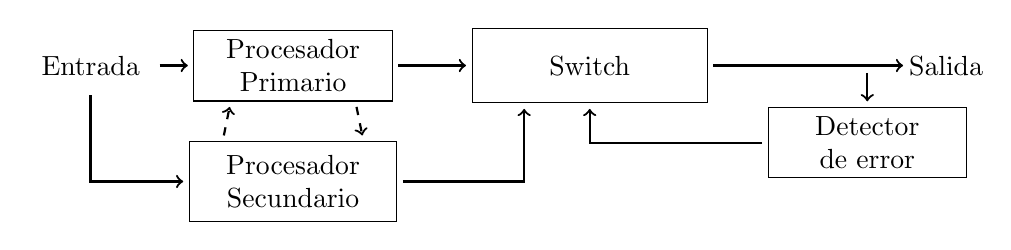
\begin{tikzpicture}[node distance=1cm, auto,]
  % definicion de estilos
  %Define style for boxes
   \tikzset{
   cuadro/.style={
           rectangle,
           draw=black,
           text width=6.5em,
           minimum height=2em,
           text centered},
    % Define arrow style
    arrow/.style={
           ->,
           thick,
           shorten <=2pt,
           shorten >=2pt,}	
    }
  \tikzstyle{circulo} = [draw, fill=black, circle, node distance=1cm, minimum size=5pt, inner 
sep=3pt]
    
  % Gráfico
  \node[inner sep=5pt] (entrada) {Entrada};
  \node[cuadro, right=0.5cm of entrada] (prim) {Procesador Primario};
  \node[cuadro, inner sep=5pt,below=0.5cm of prim] (secu) {Procesador Secundario};
  \node[cuadro, inner sep=10pt, right=1cm of prim] (selec) {Switch};
  \node[inner sep=0pt, right=2cm of selec](ghost1){};
  \node[cuadro, below=0.5cm of ghost1](detector) {Detector de error};
  \node[inner sep=0pt, right=0.5cm of ghost1] (salida) {Salida};
  
  \draw[arrow] (entrada)--(prim);
  \draw[arrow] (entrada)|-(secu);
  \draw[arrow, dashed] (prim.-30) -- (secu.30);
  \draw[arrow, dashed] (secu.150) -- (prim.-150);
  \draw[arrow] (prim)--(selec);
  \draw[arrow] (secu)-|(selec.-150);
  \draw[arrow] (detector)-|(selec);
  \draw[arrow] (selec)--(salida);
  \draw[arrow] (ghost1)--(detector);
 \end{tikzpicture}
 \caption{Representación del proceso pares}
 \label{fig:repPares}
\end{figure}

\end{comment}

\subsubsection{Diversidad de datos}
La diversidad es una técnica utilizada para mejorar la eficiencia en los checkpoint y restart, 
usando diferentes entradas por cada reinicio. Esto se basa en que las fallas en el 
\ac{SW} son dependientes de las entradas. Es poco probable que la misma falla se 
de con la misma secuencia de entrada \citep{FTDesign}.

\subsubsection{Bloques de recuperación}

Esta técnica combina las bases de la técnica de checkpoints y restart enfocada con múltiples 
versiones de un componente de \ac{SW} en el sentido de que una versión de \ac{SW} diferente es 
lanzada cada vez que se encuentra una falla. Los 
checkpoints son creados antes de que una versión de \ac{SW} se ejecuta.
La ejecución de las múltiples versiones pueden ser 
secuencial o paralelas dependiendo de la disponibilidad de la capacidad de procesamiento y 
perfomance requerida \citep{SoftwareFaultToleranceATutorial}.

%La representación de esta técnica se puede observar en el figura~[AGREGAR IMAGEN].
Las 
versiones son diferentes implementaciones de un mismo programa. Solo una de estas versiones provee 
la salida del sistema. Si un error es detectado por el test de aceptación, se vuelve hacia atrás, 
se retoma el último checkpoint, y se vuelve a ejecutar el módulo de \ac{SW} pero con una 
versión diferente a la que se ejecutó anteriormente \citep{FTDesign}.  	

Los checks del test de aceptación deben mantenerse simples para mantener la velocidad de la 
ejecución \citep{FTDesign}.

\begin{comment}
\begin{figure}[h]
 \centering
 \begin{tikzpicture}[node distance=1cm, auto,]
  % definicion de estilos
  %Define style for boxes
   \tikzset{
   cuadro/.style={
           rectangle,
           draw=black,
           text width=6.5em,
           minimum height=2em,
           text centered},
    % Define arrow style
    arrow/.style={
           ->,
           thick,
           shorten <=2pt,
           shorten >=2pt,}	
    }
       
  \tikzstyle{circulo} = [draw, fill=black, circle, node distance=1cm, minimum size=5pt, inner 
sep=3pt]
    
  % Gráfico
  \node[inner, sep=5pt] (input1){Entrada 1};
  \node[inner, sep=5pt, below=0.5cm of input1] (input2){Entrada 2};
  \node[inner, sep=5pt, below=0.5cm of input2] (puntos1){...};
  \node[inner, sep=5pt, below=0.5cm of puntos1] (inputn){Entrada n};
  \node[cuadro, right=0.5cm of input1] (version1){Versión 1};
  \node[cuadro, right=0.5cm of input2] (version2){Versión 2};
  \node[inner, sep=5pt, right=2cm of puntos1](puntos2){...};
  \node[cuadro, right=0.5cm of inputn] (versionn){Version n};
  
  \node[cuadro, above=1cm of version1] (check) {Memoria Checkpoint};
  \node[cuadro, right=1cm of version2] (switch) {Swith n a 1};
  \node[inner, sep=0pt, right=1cm of switch](ghost1){};
  \node[cuadro, below=0.5cm of ghost1](test){Test de aceptación};
  
  \node[inner, sep=0pt, right=0.5cm of ghost1](output){Salida};
 
  %Arrows
  \draw[arrow] (input1)--(version1);
  \draw[arrow] (input2)--(version2);
  \draw[arrow] (inputn)--(versionn);
  \draw[arrow] (version1)-|(switch.west);
  \draw[arrow] (version2)--(switch);
  \draw[arrow] (versionn)-|(switch.west);
  \draw[arrow] (ghost1)--(test);
  \draw[arrow] (switch)--(output);
  
  \draw[arrow, dashed] (check.-40) -- (version1.30);
  \draw[arrow, dashed] (version1.150) -- (check.-145);
  
  

 \end{tikzpicture}
 \caption{Configuración de bloques de recuperación}
 \label{fig:repPares}
\end{figure}
\end{comment}

%\subsubsection{Programación N-version}

%\subsubsection{Programación N-Auto Checking}


%\include{secciones/AreaDeEstudio}
%\section*{Datos}
\label{sec:datos}
%\section*{Metodología}
\label{sec:metodologia}
%\include{secciones/Resultados}
%\include{secciones/Discusion}

% ----------------------------------------------------------------------------------------------

\newpage
\nocite{*}
\bibliography{biblio.bib}
%\bibliographystyle{apalike}	
\bibliographystyle{plainnatesp.bst}
\addcontentsline{toc}{chapter}{Bibliograf\'ia}

%------------------------------------------------------------------------------
% EN CASO DE TENER APÉNDICES, DESCOMENTAR A CONTINUACIÓN
% \appendix
% \include{secciones/Apendice}

\newpage
$\ $
\thispagestyle{empty} % para que no se numere esta pagina
\newpage
$\ $
\thispagestyle{empty}
 
\end{document}

